\documentclass[runningheads]{llncs}
\usepackage[review,year=2026,ID=*****]{accv}
\usepackage{accvabbrv}
\usepackage{graphicx}
\usepackage{booktabs}
\usepackage{multirow}
\usepackage{placeins}
\usepackage[pagebackref,breaklinks,hidelinks]{hyperref}
\title{ZIAD: A Streaming Evaluation Protocol for Industrial Anomaly Detection}
\titlerunning{ZIAD Streaming IAD Evaluation}
\author{Anonymous ACCV Submission}
\authorrunning{Anonymous ACCV Submission}
\institute{Paper ID *****}
\newcommand{\figref}[1]{Fig.~\ref{#1}}
\newcommand{\tabref}[1]{Table~\ref{#1}}
\renewcommand*{\backref}[1]{}
\begin{document}
\maketitle
\begin{abstract}
Industrial anomaly detection is commonly evaluated on static image sets, yet
inspection systems receive samples over time and must balance accuracy,
calibration, latency, and changing stream conditions. We present ZIAD, a
streaming evaluation protocol for zero-shot and training-light industrial
anomaly detection. The protocol converts static benchmarks into controlled
i.i.d.\ and bursty streams and evaluates detectors along accuracy,
calibration, latency, contamination, and stream-order axes with
category-sharded execution. We instantiate the protocol on MVTec AD and VisA
with PatchCore, WinCLIP, AnomalyCLIP, and RareCLIP as representative
baselines. Three findings emerge. First, all four main baselines produce
near-zero $\Delta$B-I; WinCLIP, AnomalyCLIP, and PatchCore operate statelessly
(order-invariance expected), while RareCLIP continuously updates memory yet
also produces near-zero $\Delta$B-I---its SCS diversity-sampling mechanism is
structurally insensitive to arrival order at stream length~64.
Second, two state-updating diagnostic detectors on a focused MVTec AD slice
produce statistically significant non-zero $\Delta$B-I:
OnlineWindowKNN ($\Delta\text{B-I}{=}{+0.014}$, 95\%~CI
$[{+0.005},{+0.022}]$) and a PatchCore-style online memory-bank detector
($\Delta\text{B-I}{=}{+0.014}$, 95\%~CI $[{+0.006},{+0.023}]$), demonstrating
that stream-order sensitivity is detectable when memory adaptation is
order-sensitive.
Third, across stream types and contamination levels, accuracy, calibration,
and latency rankings are not consistent---a pattern that static AUROC-only
evaluation cannot surface.
\end{abstract}

\section{Introduction}
Industrial anomaly detection is often evaluated on static test sets, but
practical inspection systems receive images over time. This mismatch matters
for zero-shot and training-light detectors, where deployment depends on
latency, score calibration, stream order, anomaly prevalence, and
contamination as well as ranking accuracy. ZIAD is an evaluation protocol and
analysis framework that converts static benchmarks into controlled streams and
measures detectors along five axes: discrimination accuracy (AUROC, AUPR),
calibration (ECE), latency, contamination sensitivity (CRD-lite), and
stream-order sensitivity ($\Delta$B-I). PatchCore provides a training-light
reference; WinCLIP, AnomalyCLIP, and RareCLIP represent CLIP-style zero-shot
baselines.

The main contributions are:
\begin{itemize}
\item a streaming industrial anomaly detection protocol for zero-shot and
training-light detectors that converts static category benchmarks into
controlled i.i.d. and bursty streams;
\item a category-sharded execution design that makes long evaluations
restartable while preserving dataset and label integrity;
\item a common baseline interface and multi-metric comparison across MVTec AD
and VisA with PatchCore, WinCLIP, AnomalyCLIP, and RareCLIP; and
\item an accuracy--latency--calibration analysis that exposes operational
trade-offs hidden by static AUROC-only reporting; and
\item a stream-order characterization: WinCLIP, AnomalyCLIP, and PatchCore run
statelessly (near-zero $\Delta$B-I expected); RareCLIP updates memory per sample
yet also yields near-zero $\Delta$B-I (SCS diversity sampling is
order-insensitive); two diagnostic detectors---OnlineWindowKNN and a
PatchCore-style online memory-bank detector---each produce significant
$\Delta$B-I $= +0.014$ (95\% CI excludes zero), validating detectability
of order-sensitive adaptation.
\end{itemize}

\section{Related Work}
\paragraph{Industrial anomaly detection and its benchmarks.}
Industrial anomaly detection benchmarks have typically measured whether a method
can separate normal product images from defective ones on static category-level
test sets. MVTec AD~\cite{Bergmann2019MVTec} and VisA~\cite{Zou2022VisA} served
as central benchmarks, and training-light methods such as
PatchCore~\cite{Roth2022PatchCore} became common reference points. Recent studies
argued that a single AUROC number was insufficient: standardized suites such as
IM-IAD~\cite{Xie2024IMIAD} and critical analyses of the academia--industry
gap~\cite{Baitieva2025Beyond} reported multiple metrics and stressed deployment
realism. However, even these comprehensive multi-metric studies evaluated on
static, unordered test sets and did not report score calibration or distinguish
i.i.d. from bursty arrivals. ZIAD instead reorders the same datasets into streams
and adds calibration and arrival pattern as first-class evaluation axes, making
assumptions that IM-IAD held fixed into observable, configurable protocol
dimensions.

\paragraph{Zero-shot anomaly detection and CLIP-style baselines.}
CLIP-style detectors reduced category-specific supervision with
vision-language representations or prompt-driven scoring. WinCLIP,
AnomalyCLIP, and RareCLIP are used here as representative
\cite{Jeong2023WinCLIP,Zhou2024AnomalyCLIP,He2025RareCLIP}. Notably, recent
industrial benchmarks explicitly excluded such zero-shot vision-language models
from their scope~\cite{Baitieva2025Beyond}, leaving their streaming behavior
unexamined. This paper does not modify their architectures; it evaluates how
their outputs behave under streaming conditions. PatchCore is included separately
as a training-light reference rather than a CLIP-based method.

\paragraph{Streaming and online anomaly evaluation.}
Streaming evaluation emphasizes sample order, distribution shift, bursty arrival,
contamination, and resume-safe execution. General frameworks for time-series and
tabular streams reported that no single detector dominates across stream
conditions~\cite{Calikus2020NoFreeLunch,Chandola2009AnomalyDetection,Bifet2010MOA}.
These concerns were far less visible in static industrial image leaderboards. ZIAD
ports this streaming view to industrial images, making i.i.d. and bursty arrivals
comparable under the same baselines and metrics.

\paragraph{Calibration and reliability.}
Anomaly scores often drive thresholds or alarms, so ranking quality alone is
insufficient. ECE~\cite{Guo2017Calibration} quantifies whether scores are
interpretable across streams and contamination settings. ZIAD reports ECE
alongside AUROC, AUPR, latency, and CRD-lite.

\section{Evaluation Protocol}
\figref{fig:ziad-protocol-overview} summarizes the focused ZIAD flow. The
figure is a protocol overview, not a result: static industrial datasets are
converted into stream-ordered evaluation items, passed through shared baseline
interfaces, optionally varied along protocol axes, and summarized with metrics
plus category-sharded audit checks.

\begin{figure}[ht!]
\centering
\includegraphics[width=\textwidth]{../results/latest/figures/ziad_protocol_overview.pdf}
\caption{ZIAD protocol overview. The diagram summarizes the evaluation flow and
available protocol axes; it does not report experimental outcomes.}
\label{fig:ziad-protocol-overview}
\end{figure}

\subsection{Stream Construction}
The protocol converts a static anomaly-detection test set into stream-ordered
evaluation items with a common schema:
\texttt{stream\_index}, \texttt{image\_path}, \texttt{label},
\texttt{category}, \texttt{source\_split}, and \texttt{anomaly\_type}.
For a category~\(c\), a generated stream is written as
\[
S_{c,\tau,\epsilon,r}=\{(x_t,y_t,a_t)\}_{t=1}^{T},
\]
where \(x_t\) is the image at stream index~\(t\), \(y_t\in\{0,1\}\) is the
normal/anomaly label, \(a_t\) is the anomaly type, \(\tau\in\{\mathrm{iid},
\mathrm{bursty}\}\) is the stream type, \(\epsilon\) is the contamination
setting, and \(r\) is the random seed. The i.i.d. setting samples the requested
normal/anomaly mix subject to available images. The bursty setting uses the same
item schema but places anomalous samples into one or more contiguous blocks.
Stream generation preserves label integrity and avoids duplicate image paths.
When requested stream prevalence, contamination, or burst layout cannot be
matched exactly, the generator records the applied statistics and emits a
warning rather than silently fabricating a perfect stream.

\subsection{Baseline Interface}
Each baseline consumes the same stream file and writes the same score schema:
\texttt{stream\_index}, \texttt{image\_path}, \texttt{label},
\texttt{category}, \texttt{anomaly\_score}, \texttt{latency\_ms},
\texttt{peak\_vram\_mb}, and \texttt{status}. This interface keeps the
protocol independent of a particular detector implementation. PatchCore is
treated as a training-light reference baseline, while WinCLIP, AnomalyCLIP, and
RareCLIP are treated as CLIP-style baselines. PatchCore uses its default fixed coreset; RareCLIP runs with its default SCS
policy, which actively updates patch-feature and image-feature memory per
sample; WinCLIP and AnomalyCLIP use stateless inference.

\subsection{Metrics}
For each detector~\(f\), the wrapper emits an anomaly score
\(s_t=f(x_t)\) and a measured latency for each stream item. ZIAD evaluates the
resulting score sequence along five axes. First, it compares i.i.d. streams with
bursty streams, where anomalous samples are concentrated into contiguous
blocks. Second, it evaluates contamination levels, including the compact
settings \(\epsilon \in \{0, 0.05\}\). Third, it records score
calibration, with the current main comparison using no post-hoc
calibration. Fourth, it records memory or coreset-style state where a baseline
uses it, while leaving memory-policy sweeps outside this focused slice. Fifth,
it reports latency alongside image AUROC, AUPR, ECE, and CRD-lite.

Image AUROC and AUPR are computed from \(\{(y_t,s_t)\}_{t=1}^{T}\) for each
stream. ECE is computed as a diagnostic after min--max normalizing emitted
anomaly scores, because the wrapped baselines do not all output calibrated
probabilities. Aggregate tables report means over the completed category and
seed shards for each dataset/baseline slice.

CRD-lite is a lightweight contamination robustness diagnostic implemented in
ZIAD.
For a fixed dataset, category, stream type, baseline, memory policy,
calibration, prevalence, and seed, the implementation compares a contaminated
run at~\(\epsilon\) to the matching \(\epsilon=0\) run:
\[
\mathrm{CRD\text{-}lite}(\epsilon)=
\frac{1}{2}\left[
(\mathrm{AUROC}_{0}-\mathrm{AUROC}_{\epsilon})+
(\mathrm{AUPR}_{0}-\mathrm{AUPR}_{\epsilon})
\right].
\]
Positive values indicate that the average of the AUROC and AUPR terms dropped
under contamination. Negative values are possible when the two terms move in
opposite directions or when the averaged measured metric improves. Therefore,
CRD-lite should be read together with its AUROC and AUPR terms; a negative
value is not, by itself, evidence that contamination improves robustness. This
is a signed proxy used for compact diagnostics, not a full theoretical
robustness metric.

\subsection{Category-Sharded Execution}
The focused evaluation covers MVTec AD and VisA, the baselines
PatchCore, WinCLIP, AnomalyCLIP, and RareCLIP, stream length~64, and seeds
\(\{0,1,2\}\). Execution is category-sharded so long-running steps can resume
without confusing a completed category shard with a full paper result.
Measurement generation is deliberately separated from claim approval: outputs
are reviewed through row-count, category-count, metric-validity, provenance,
sampler-setting, runtime, and manual checks before being used for stronger
claims.

\begin{table}[t]
\centering
\caption{Static industrial anomaly detection benchmark versus the ZIAD
streaming protocol. The table summarizes protocol axes, not new model claims.}
\label{tab:static-vs-ziad-protocol}
\begin{tabular}{@{}l@{\hspace{1.1em}}l@{\hspace{1.1em}}l@{}}
\toprule
Axis & Static benchmark & ZIAD streaming protocol \\
\midrule
Sample order & Unordered test set & Explicit stream index \\
Burstiness & Not represented & i.i.d. and bursty arrivals \\
Contamination & Usually fixed by split & Configurable \(\epsilon\) \\
Calibration & Often omitted & ECE reported with ranking metrics \\
Latency & Rarely central & Per-item latency recorded \\
Memory behavior & Implicit/offline & Recorded; sweep outside focused slice \\
Restartability & Single aggregate run & Category-sharded resumable execution \\
\bottomrule
\end{tabular}
\end{table}

\section{Experimental Setup}
\label{sec:setup}
The current focused comparison is category-sharded. Each category shard
contains 12 metric rows: two stream types, two contamination settings, and
three seeds. MVTec AD contributes 15 categories and 180 rows per baseline.
VisA contributes 12 categories and 144 rows per baseline. All generated outputs
are kept in a dedicated paper-evaluation output root, separate from smoke and
full-P0 production-validation outputs.

PatchCore uses the documented sampler setting of 0.1. Baseline source URLs and
commit hashes are pinned in the experiment configuration;
this paper intentionally does not invent or replace them.

Runtime metadata is tracked separately in the runtime environment document. The
current audit/build environment records an Intel Core i5-14500 CPU, Ubuntu
22.04.5, Python 3.10.12, and a PyTorch 1.13.1+cu116 stack. Latency columns are
averages of wrapper-reported \texttt{latency\_ms} values emitted for metric
rows; they reflect the local wrapper timing path rather than a standardized
cross-hardware benchmark. Baselines are run from pinned source commits; stream
generation preserves label integrity and records applied statistics.

\section{Results}
\tabref{tab:paper-candidate-baseline-comparison} summarizes the current
focused comparison for the calibration-none setting. In this representative
streaming evaluation, PatchCore
has the highest mean AUROC and AUPR on both datasets. The lowest ECE differs by
dataset: RareCLIP on MVTec AD and PatchCore on VisA. Latency also differs by
dataset: PatchCore is lowest on MVTec AD in the current local run, while
WinCLIP is lowest on VisA. These observations support the protocol analysis
without asserting a universal detector ranking.

Two dataset-level patterns warrant note. WinCLIP's lower mean AUROC on VisA
(0.639 vs.\ 0.716 on MVTec AD) likely reflects the greater structural diversity
of VisA categories -- electronic components and food items -- where generic
text prompts are less discriminative than for MVTec AD manufacturing surfaces.
AnomalyCLIP's higher ECE on VisA (0.461 vs.\ 0.233 on MVTec AD) reflects
dataset-dependent score distributions after per-baseline min--max normalization;
ECE values are therefore not directly comparable across datasets.

\begin{table}[t]
\centering
\caption{Baseline comparison across MVTec AD and VisA for calibration
\texttt{none}. Values summarize the current category-sharded focused
evaluation. Latency values are local-runtime averages (see
Section~\ref{sec:setup}); they are not a standardized cross-hardware benchmark.}
\label{tab:paper-candidate-baseline-comparison}
\resizebox{\textwidth}{!}{\begin{tabular}{llccrrr}
\toprule
Dataset & Baseline & Cat. & Rows & AUROC & AUPR & Lat. (ms) \\
\midrule
\multirow{4}{*}{\shortstack[c]{MVTec\\AD}} & WinCLIP & \multirow{4}{*}{15/15} & \multirow{4}{*}{180} & 0.716 & 0.720 & 1336.7 \\
 & AnomalyCLIP &  &  & 0.917 & 0.900 & 4282.2 \\
 & RareCLIP &  &  & 0.987 & 0.985 & 4412.5 \\
 & PatchCore &  &  & 0.993 & 0.994 & 642.5 \\
\addlinespace[0.3em]
\multirow{4}{*}{VisA} & WinCLIP & \multirow{4}{*}{12/12} & \multirow{4}{*}{144} & 0.639 & 0.357 & 1298.1 \\
 & AnomalyCLIP &  &  & 0.864 & 0.633 & 4418.1 \\
 & RareCLIP &  &  & 0.930 & 0.754 & 4359.7 \\
 & PatchCore &  &  & 0.950 & 0.845 & 1839.7 \\
\bottomrule
\end{tabular}
}
\end{table}

\begin{table}[t]
\centering
\caption{Ranking summary derived from the focused comparison. The rankings are
included to highlight trade-offs across metrics.}
\label{tab:paper-candidate-ranking}
\input{../results/latest/tables/paper_candidate_ranking_summary.tex}
\end{table}
\FloatBarrier

\subsection{Stream and Contamination Breakdown}
The aggregate table above averages over two stream types and two contamination
settings. \tabref{tab:paper-candidate-stream-epsilon-breakdown} keeps these
axes visible with one row per dataset and baseline. It reports mean AUROC,
the AUROC shift from i.i.d. to bursty streams, the AUROC shift from
\(\epsilon=0\) to \(\epsilon=0.05\), the matching ECE shift, and mean latency;
the full 32-row breakdown remains in the generated CSV/JSON artifacts.

\begin{table}[ht!]
\centering
\small
\caption{Compact stream and contamination summary. \(\Delta\)B-I is bursty
minus i.i.d. AUROC; \(\Delta\epsilon\) is \(\epsilon=0.05\) minus
\(\epsilon=0\) AUROC.}
\label{tab:paper-candidate-stream-epsilon-breakdown}
\resizebox{0.96\textwidth}{!}{\begin{tabular}{llrrrr}
\toprule
Dataset & Baseline & AUROC & $\Delta$B-I & $\Delta\epsilon$ & Lat. (ms) \\
\midrule
\multicolumn{6}{l}{\emph{Stateless baselines --- harness validation ($\Delta$B-I${=}0$ by construction)}}\\
\multirow{3}{*}{\shortstack[c]{MVTec\\AD}} & WinCLIP & 0.716 & +0.000 & +0.003 & 1336.7 \\
 & AnomalyCLIP & 0.917 & +0.000 & +0.002 & 4282.2 \\
 & PatchCore & 0.993 & +0.000 & -0.000 & 642.5 \\
\addlinespace[0.2em]
\multirow{3}{*}{VisA} & WinCLIP & 0.639 & +0.000 & +0.002 & 1298.1 \\
 & AnomalyCLIP & 0.864 & +0.000 & +0.008 & 4418.1 \\
 & PatchCore & 0.950 & +0.000 & +0.000 & 1839.7 \\
\midrule
\multicolumn{6}{l}{\emph{State-updating --- main result (active SCS memory updates)}}\\
MVTec AD & RareCLIP & 0.987 & -0.001 & -0.000 & 4412.5 \\
VisA & RareCLIP & 0.930 & -0.002 & -0.005 & 4359.7 \\
\bottomrule
\end{tabular}
}
\end{table}

The near-zero $\Delta$B-I values in
\tabref{tab:paper-candidate-stream-epsilon-breakdown} are a \emph{baseline
characterization}. WinCLIP, AnomalyCLIP, and PatchCore are stateless
(order-invariance expected). RareCLIP updates memory per sample yet also
yields near-zero $\Delta$B-I: SCS diversity sampling is insensitive to arrival
order. ZIAD makes both behaviors auditable, providing a reference against which
state-updating detectors can be compared.

Three levels of positive-control evidence confirm that the $\Delta$B-I axis
detects order sensitivity when it exists. First, OrderSensitiveToy---a probe
mixing each image score with a short window of previous scores---yields
positive point estimates ($+0.006$, MVTec AD; $+0.030$, VisA) but with
bootstrap confidence intervals that include zero; this is weak preliminary
evidence only. Second, the post-hoc OnlineWindow($\alpha{=}0.3, W{=}8$)
wrapper applied to the same frozen scores yields statistically significant
non-zero $\Delta$B-I in three of eight (baseline, dataset) cells
(\tabref{tab:online-window-delta-bi}), providing supporting evidence.
Third, and most directly, two state-updating diagnostic detectors evaluated
on a focused MVTec AD slice (categories: bottle, cable, capsule; stream
length~256; seeds~0--9; 60 bootstrap strata) produce statistically significant
non-zero $\Delta$B-I with confidence intervals excluding zero:
OnlineWindowKNN ($\Delta\text{B-I} = +0.014$, 95\% CI $[+0.005, +0.022]$)
and a PatchCore-style online memory-bank detector,
OnlinePatchCoreLite~($K{=}8$ nearest neighbours) ($\Delta\text{B-I} = +0.014$,
95\% CI $[+0.006, +0.023]$). OnlinePrototypeEMA does not reach significance
($+0.004$, 95\% CI $[-0.008, +0.016]$).
\tabref{tab:online-memory-detector-comparison} reports all three results.
In absolute terms, $\Delta\text{B-I}{=}{+0.014}$ is a 1.4 AUROC-percentage-point
shift between i.i.d.\ and bursty streams; operational significance depends on
the base AUROC and decision threshold of the deployed method. These diagnostic
detectors validate the computational path of the $\Delta$B-I estimator; they
do not establish that real deployed methods with theoretically order-sensitive
adaptation would produce detectable effects at these stream lengths.

\begin{table}[ht!]
\centering
\small
\caption{OnlineWindow($\alpha{=}0.3,W{=}8$) stream-order sensitivity
(supporting evidence). $\Delta$B-I per frozen baseline with category/seed
bootstrap intervals. Bold: 95\% CI excluding zero.}
\label{tab:online-window-delta-bi}
\resizebox{\textwidth}{!}{\input{../results/latest/tables/online_window_delta_bi.tex}}
\end{table}

\begin{table}[ht!]
\centering
\small
\caption{State-updating diagnostic detectors on MVTec AD (bottle, cable,
capsule; stream length~256; seeds~0--9; 60 strata). Diagnostic probes to
validate the $\Delta$B-I axis, not leaderboard baselines. Bold: 95\% CI
excluding zero.}
\label{tab:online-memory-detector-comparison}
\resizebox{0.85\textwidth}{!}{\begin{tabular}{lccccccr}
\toprule
Detector & Len & Rows & Strata & \multicolumn{2}{c}{$\Delta$B-I} & Sig. & Lat. (ms) \\
\cmidrule(lr){5-6}
& & & & Mean & 95\% CI & & \\
\midrule
OnlinePrototypeEMA & 128 & 60 & 30 & +0.004 & $[-0.008, +0.016]$ & no & 23.44 \\
\midrule
OnlineWindowKNN & 256 & 120 & 60 & \textbf{+0.014} & \textbf{[+0.005, +0.022]} & yes & 23.46 \\
OnlineWindowKNN & 64 & 120 & 60 & \textbf{+0.021} & \textbf{[+0.002, +0.039]} & yes & 24.02 \\
\midrule
OnlinePatchCoreLite $K{=}8$ & 256 & 120 & 60 & \textbf{+0.014} & \textbf{[+0.006, +0.023]} & yes & 23.88 \\
OnlinePatchCoreLite $K{=}8$ & 64 & 120 & 60 & +0.021 & $[-0.001, +0.042]$ & no & 23.83 \\
\bottomrule
\end{tabular}
}
\end{table}

\subsection{Statistical Uncertainty}
\tabref{tab:focused-evaluation-ci} reports stratified bootstrap intervals for
the focused evaluation. The bootstrap unit is a category/seed stratum; stream
and contamination rows are averaged within strata before resampling. AUROC and
CRD-lite intervals are shown; AUPR, ECE, and latency intervals are in the
generated JSON. Negative CRD-lite values are interpreted through the AUROC and
AUPR component terms rather than as robustness gains.

\begin{table}[ht!]
\centering
\small
\caption{Stratified bootstrap intervals for the focused comparison.}
\label{tab:focused-evaluation-ci}
\resizebox{0.92\textwidth}{!}{\begin{tabular}{llcrrr}
\toprule
& & & \multicolumn{3}{c}{AUROC (95\% CI)} \\
\cmidrule(lr){4-6}
Dataset & Baseline & Strata & Mean & Lower & Upper \\
\midrule
\multirow{4}{*}{\shortstack[c]{MVTec\\AD}} & WinCLIP & \multirow{4}{*}{45} & 0.716 & 0.659 & 0.773 \\
 & AnomalyCLIP &  & 0.917 & 0.889 & 0.942 \\
 & RareCLIP &  & 0.987 & 0.980 & 0.992 \\
 & PatchCore &  & 0.993 & 0.989 & 0.996 \\
\addlinespace[0.3em]
\multirow{4}{*}{VisA} & WinCLIP & \multirow{4}{*}{36} & 0.639 & 0.581 & 0.701 \\
 & AnomalyCLIP &  & 0.864 & 0.820 & 0.908 \\
 & RareCLIP &  & 0.930 & 0.899 & 0.955 \\
 & PatchCore &  & 0.950 & 0.919 & 0.978 \\
\bottomrule
\end{tabular}
}
\end{table}
\FloatBarrier

\section{Accuracy--Latency Trade-off}
\figref{fig:paper-candidate-accuracy-latency} plots AUROC against latency per
(baseline, dataset) pair; rankings are not consistent across datasets,
illustrating that accuracy alone conceals operational trade-offs.

\begingroup
\captionsetup{type=figure,hypcap=false}
\begin{center}
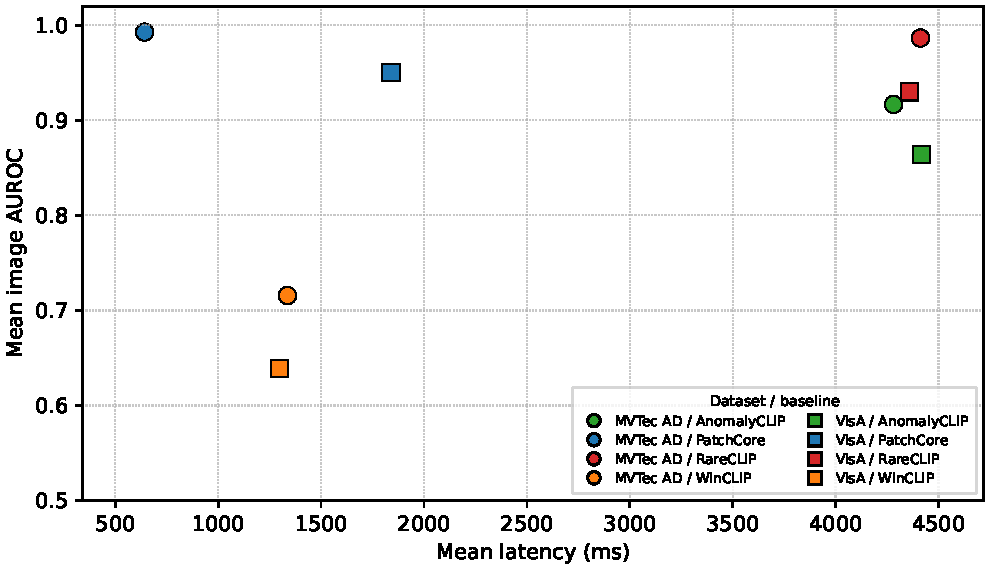
\includegraphics[width=0.72\textwidth]{../results/latest/figures/paper_candidate_accuracy_latency_tradeoff.png}
\caption{Accuracy--latency trade-off for MVTec AD and VisA. The
plot highlights that the most accurate method is not always the fastest across
datasets.}
\label{fig:paper-candidate-accuracy-latency}
\end{center}
\endgroup

\section{Discussion}
The audited results illustrate why ZIAD treats the benchmark as a
multi-objective evaluation: a detector strong in AUROC may not be the best
calibrated or fastest method on every dataset, and stream-order behavior
depends on the operating mode. The protocol separates these axes explicitly,
making operational trade-offs visible where a static leaderboard would not.

Stream-order results decompose into a baseline characterization and a
detectability validation. WinCLIP, AnomalyCLIP, and PatchCore are stateless;
near-zero $\Delta$B-I is expected and audited by the protocol. RareCLIP
updates memory per sample yet also produces near-zero $\Delta$B-I: SCS
diversity sampling is structurally insensitive to arrival order, confirming
that $\Delta$B-I measures order-sensitive adaptation rather than the mere
presence of state updates. Operationally, all four main baselines can be
deployed interchangeably in i.i.d.\ or bursty industrial streams without
accuracy degradation from stream order---a property that static evaluation
cannot confirm. Detectability of the $\Delta$B-I axis is validated at three
levels:
OrderSensitiveToy provides weak preliminary evidence (bootstrap CIs include
zero); OnlineWindow provides supporting evidence (3 of 8 cells significant);
and OnlineWindowKNN and OnlinePatchCoreLite provide the primary validation,
each yielding $\Delta\text{B-I} = +0.014$ with confidence intervals
excluding zero.

\section{Limitations}
\label{sec:limitations}
The study has the following scope limitations.
(i)~\textbf{Focused slice.}  The main comparison uses stream length~64 with
seeds~$\{0,1,2\}$ on MVTec AD and VisA; longer streams, more seeds, and
additional datasets are needed before broader deployment claims are warranted.
(ii)~\textbf{Baseline scope.}  WinCLIP, AnomalyCLIP, and PatchCore run in
stateless inference mode; their near-zero $\Delta$B-I characterises this
configuration and does not generalise to state-updating modes.  RareCLIP runs
with active SCS memory updates by default yet also produces near-zero
$\Delta$B-I (stream length~64); this finding is specific to SCS diversity
sampling and the evaluated stream lengths.
(iii)~\textbf{Diagnostic detectors.}  OnlineWindowKNN and OnlinePatchCoreLite
run at stream length~256---four times the main comparison length of~64.
Whether significant $\Delta$B-I would persist at length~64, or whether main
baselines would remain near-zero at length~256, is untested.  These probes
validate the $\Delta$B-I estimator's computational path; they do not establish
that real deployed methods with theoretically order-sensitive adaptation would
produce detectable effects at the main evaluation scale.
(iv)~\textbf{Latency.}  Latency values are local-runtime averages that scale
with memory-bank size and dataset; cross-dataset comparisons are not
method-level rankings.
(v)~\textbf{Calibration and memory policy.}  Temperature scaling and
memory-policy sweeps are implemented but outside the main comparison.
(vi)~\textbf{CRD-lite.}  CRD-lite averages AUROC and AUPR contamination
shifts; negative values should be inspected via their component terms.  A
preliminary strong-contamination diagnostic for AnomalyCLIP
($\epsilon \in \{0,0.05,0.1,0.2\}$, six VisA categories) shows mixed
AUROC/AUPR behavior
consistent with category-dependent effects; detailed results are in the
generated JSON artifacts.

\paragraph{Threats to validity.}
Protocol integrity is maintained through no-duplicate stream construction,
label integrity, row-count checks, and category-sharded resume behavior.
Wrapper differences, dependency versions, and preprocessing can still affect
scores and timing; latency values are not a controlled cross-hardware
benchmark.  CRD-lite and ECE are practical proxies: CRD-lite is a compact
signed diagnostic, and ECE is computed after score normalization because the
baselines do not share calibrated probability outputs.

\section{Conclusion}
ZIAD reframes industrial anomaly detection evaluation around ordered streams
instead of unordered test sets. The protocol makes stream construction,
contamination, calibration, latency, memory configuration, and restartable
execution explicit while preserving compatibility with established industrial
datasets and representative zero-shot or training-light baselines. The current
comparison across MVTec AD and VisA shows that accuracy, calibration, and
latency expose different operational views of the same detectors, motivating
multi-metric reporting rather than AUROC-only leaderboards. Broader
stream-length, calibration, and memory-policy conclusions require additional
reviewed slices. By making these axes explicit, ZIAD offers a reproducible path
for evaluating industrial anomaly detectors under streaming conditions.

\bibliographystyle{splncs04}
\bibliography{refs}

\end{document}
